%!TEX program = xelatex
\documentclass[cn,blue,normal,founder,11pt]{elegantnote}

\hypersetup{
			pdftitle={图论第二次作业},
			pdfauthor={李徐瑾}
}

\usepackage{amssymb}
\usepackage{mathtools}
\let\Bbbk\undefined
\usepackage[complete,subscriptcorrection,slantedGreek]{mtpro2}
\let\qedhere\undefined
\newcommand{\calO}{\mathcal{O}}
\renewcommand{\qed}{\(\hfill\square\)}
\renewcommand{\proofname}{\normalfont\bfseries\color{ecolor}解}

\title{图论第二次作业}
\institute{数数学科学学院}
\author{李徐瑾\quad 202021110109}
\date{\zhtoday}

\begin{document}

\maketitle

\centerline{\includegraphics[scale=0.16]{image/UESTC_cp.pdf}}
\section{习题四}

\begin{example}
判断图\ref{fig:4.1}所示的四个图是否可以一笔画.
\begin{figure}[h]
  \centering
  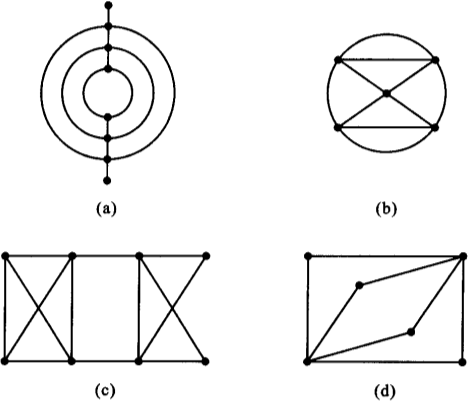
\includegraphics[scale=0.50]{image/ex1.pdf}
  \caption{}
  \label{fig:4.1}
\end{figure}
\end{example}

\begin{proof}
(a) 不可以;(b) 可以;(c) 可以;(d) 可以.
\end{proof}

\begin{example}
\begin{enumerate}[(1)]
\item 画一个有Euler闭迹和Hamilton圈的图;
\item 画一个有Euler闭迹但没有Hamilton圈的图;
\item 画一个有Hamilton圈但没有Euler闭迹的图;
\item 画一个既没有Euler闭迹也没有Hamilton圈的图.
\end{enumerate}
\end{example}

\begin{proof}
\begin{enumerate}[(1)]
\item 完全图\(K_3\);
\item 两个恰好有\(1\)个公共顶点的圈;
\item 完全图\(K_4\);
\item Peterson图.
\end{enumerate}
\end{proof}

\begin{example}
设\(n\)阶无向简单图\(G\)有\(m\)条边. 证明: 若
\[m\geqslant C_{n-1}^2+2,\]
则\(G\)是Hamilton图.
\end{example}

\begin{proof}
反证法. 设\(G\)是\(n\geqslant 3\)的非H简单图. 对于某个正整数\(m<n/2\),\(G\)度弱于\(C_{m,n}\). 已知
\[\sum_{v\in V(G)}d(v)=2|E(G)|,\]
因此
\begin{align*}
|E(G)|&\leqslant|E(C_{m,n})|\\
&=\frac{1}{2}[m^2+(n-2m)(n-m-1)+m(n-1)]\\
&=C_{n-1}^2+1-\frac{1}{2}(m-1)(m-2)-(m-1)(n-2m-1)\\
&\leqslant C_{n-1}^2+1.
\end{align*}
这是矛盾的.
\end{proof}

\begin{example}
证明: 若\(G\)没有奇点,则存在边不重的圈\(C_1,C_2,\cdots,C_m\)使得
\[E(G)=\bigcup_{i=1}^k E(Q_i).\]
\end{example}

\begin{proof}
因为\(G\)没有奇点,所以\(G\)的每个非平凡连通分支都是Euler图. 因此,\(G\)的每个连通分支的边集均可表示成边不重的圈的并. 故图\(G\)的边集可表示成边不重的圈的并.
\end{proof}

\begin{example}
证明: 若\(G\)有\(2k>0\)个奇点,则存在\(k\)条边不重的迹\(Q_1,Q_2,\cdots,Q_k\)使得
\[E(G)=\bigcup_{i=1}^k E(Q_i).\]
\end{example}

\begin{proof}
假设图\(G\)是连通图. 图\(G\)的奇点记为\(\{v_i\}_{i=1}^{2k}\). 添加边\(e_i=(v_i,v_{i+1}),\forall 1\leqslant i\leqslant k\)得到图\(G^{\prime}\). 显然图\(G^{\prime}\)是Euler图. 且图\(G^{\prime}\)的边集是一条回路\(Q\). 再从回路\(Q\)中去掉边\(\{e_i\}_{i=1}^k\),得到\(k\)条边不重的迹\(Q_1,Q_2,\cdots,Q_k\). 故有
\[E(G)=\bigcup_{i=1}^k E(Q_i).\]
\end{proof}

\begin{example}
证明: 若
\begin{enumerate}[(1)]
\item \(G\)不是二连通的图,
\item 或\(G\)是具有二分类\((X,Y)\)的偶图,其中\(|X|\ne|Y|\),
\end{enumerate}
则\(G\)是非Hamilton图.
\end{example}

\begin{proof}
\begin{enumerate}[(1)]
\item 因为图\(G\)不是二连通的,因此图\(G\)包含割点\(v\)使得\(\omega(G-v)\geqslant 2\). 故图\(G\)是非Hamilton图,
\item 反证法. 若图\(G\)是Hamilton图,则其Hamilton圈必交替经过\(X\)和\(Y\)的顶点,因此\(|X|=|Y|\),这是矛盾的.
\end{enumerate}
\end{proof}

\begin{example}
证明: 若\(G\)有Hamilton路,则对于\(V\)的每个真子集\(S\),有\(\omega(G-S)\leqslant|S|+1\).
\end{example}

\begin{proof}
设\(G\)的H圈是\(C\),\(S\)是\(V\)的非空真子集.
\begin{enumerate}[(1)]
\item \(S\)中只含\(C\)中诸邻接顶点. 这时图\(G-S\)显然是一条路,因此有
\[\omega(C-S)=1;\] 
\item \(S\)中只含\(r\)个在\(C\)均不邻接的顶点. 这时图\(C-S\)有\(r\)个分支,于是
\[\omega(C-S)=r.\]
\end{enumerate}
一般而言,若\(S\)中既含有邻接的顶点又含有不邻接的顶点,则有
\[\omega(C-S)\leqslant|S|+1.\]

因为\(C-S\)是\(G-S\)的一个生成子图,故
\[\omega(G-S)\leqslant\omega(C-S)\leqslant|S|+1.\]
\end{proof}

\begin{example}
设\(G\)是有度序列\((d_1,d_2,\cdots,d_n)\)的非平凡简单图,其中\(d_1\leqslant d_2\leqslant\cdots\leqslant d_n\). 证明: 若不存在\(m<(n+1)/2\),使得\(d_m<m\)且\(d_{n-m+1}<n-m\),则\(G\)有Hamilton路.
\end{example}

\begin{proof}
增加点\(v\)使得\(v\notin V(G)\),将\(v\)与图\(G\)的所有点连接起来得到图\(G^{\prime}\). 显然图\(G\)的度序列为\((d_1+1,d_2+1,\cdots,d_n+1,n)\). 已知不存在\(m<(n+1)/2\),使得\(d_m+1<m\)且\(d_{n-m+1}+1<n-m\). 根据度序列判断定理可知,\(G^{\prime}\)是Hamilton图,因此\(G\)包含Hamilton路.
\end{proof}

\begin{example}
对于下列问题给出一个好算法:
\begin{enumerate}[(1)]
\item 构作一个图的闭包;
\item 若某图的闭包是完全图,求该图的Hamilton圈.
\end{enumerate}
\end{example}

\begin{proof}
\begin{enumerate}[\heiti{步}1]
\item 令\(G_0=G,k=0\);
\item 在\(G_k\)中求顶点\(u,v\),使得
\[d_{G_k}(u)+d_{G_k}(v)=\max\{d_{G_k}(x)+d_{G_k}(y)\mid xy\notin E(G_k)\};\]
\item 若\(d_{G_k}(u)+d_{G_k}(v)\geqslant|G|\),转到步4;否则停止,此时得到图\(G^{\prime}\)的闭包;
\item 令\(G_{k+1}=G_k+uv,k=k+1\),转到步2.
\end{enumerate}

由于总运算量为\(\calO(n^2)\),因此是好算法. 且若图\(G\)的闭包是完全图,则采用边交换技术把\(G\)的闭包中的一个Hamilton圈化为图\(G\)中的一个Hamilton圈.
\end{proof}

\section{习题五}

\begin{example}\label{ex:5.1}
\begin{enumerate}[(1)]
\item 证明: 每个\(k\)方体都有完美匹配\((k>2)\);
\item 求\(K_{2n}\)和\(K_{n,n}\)中不同的完美匹配的个数.
\end{enumerate}
\end{example}

\begin{proof}
\begin{enumerate}[(1)]
\item 由于\(k\)方体是\(k\)正则的二部图,故\(k\)方体中存在完美匹配;
\item \(K_{2n}\)和\(K_{n,n}\)中不同的完美匹配的个数分别为\((2n-1)!!\)和\(n!\).
\end{enumerate}
\end{proof}

\begin{example}
证明: 一棵树最多只有一个完美匹配.
\end{example}

\begin{proof}
反证法. 设树\(T\)存在两个完美匹配\(M_1\)和\(M_2\),则\(M_1\triangle M_2\ne\varnothing\). 易知,在树\(T(M_1\triangle M_2)\)中的每个顶点的度数均为\(2\)度. 因此树\(T\)中存在圈,这是矛盾的.
\end{proof}

\begin{example}
对每一个\(k>1\),找出一个没有完美匹配的\(k\)正则简单图的例子.
\end{example}

\begin{proof}
当\(k\)为偶数时,完全图\(K_{k+1}\)没有完美匹配的\(k\)正则简单图.

当\(k\)为奇数时,构造图\(H\)使得\(V(H)=\{v_1,v_2,\cdots,v_{2k-1}\}\)且
\begin{align*}
E(H)=&\{v_1v_2,v_1v_4,\cdots,v_1v_{2k-2},v_3v_2,\cdots,v_3v_{2k-2},\cdots,v_{2k-1}v_2,v_{2k-1}v_4,\cdots,v_{2k-1}v_{2k-2}\}\\
&\cup\{v_1v_3,v_5v_7,\cdots,v_{2k-5}v_{2k-3}\}.
\end{align*}
在\(H\)中的仅有\(\deg(v_{2k-1})=k-1\),其余顶点的度数均为\(k\). 先将\(H\)复制\(k\)次,再添加新顶点\(u\),并将\(u\)与每个\(v_{2k-1}\)连接得到图\(G\). 图\(G\)为阶数为\(k(2k-1)+1\)的\(k\)正则图.

假设\(G\)包含完美匹配\(M\). 因为\(H\)有\(2k-1\)个点,每个\(H\)中至多有\(k-1\)条边属于\(M\). 且顶点\(u\)不在任何\(H\)中,故\(|M|\leqslant k(k-1)+1\). 因此,\(M\)中包含的顶点数不超过\(2k(k-1)+2\). 当\(k>1\)时有
\[|V(G)|=k(2k-1)+1>2k(k-1)+2\geqslant 2|M|.\]
故\(M\)不是\(G\)的生成子图,矛盾. 图\(G\)不包含完美匹配.
\end{proof}

\begin{example}
证明: \(K_4\)有唯一的一个\(1\)-因子分解. 并给出\(K_8\)的一个\(1\)-因子分解.
\end{example}

\begin{proof}
因为\(K_4\)有\(3\)不同的完美匹配,且\(K_4\)的每个\(1\)-因子分解包含\(3\)个不同的完美匹配. 故\(K_4\)有唯一的一个\(1\)-因子分解. \(K_8\)的一个\(1\)-因子分解有
\[G_1=\{v_1 v_8,v_2 v_7,v_3 v_6,v_4 v_5\},\quad\forall v_i\in V(K_8).\]
\end{proof}

\begin{example}
求\(K_{3,3}\)和\(K_6\)的\(1\)-因子分解的数目.
\end{example}

\begin{proof}
根据习题\ref{ex:5.1}的结论可知,\(K_{3,3}\)和\(K_6\)的\(1\)-因子分解的数目分别为\(6\)个和\(15\)个.
\end{proof}

\begin{example}
证明: \(K_{6n-2}\)有一个\(3\)-因子分解.
\end{example}

\begin{proof}
由于\(K_{6n-2}\)可分解为\(6n-3\)个边不重的\(1\)-因子的并,且\(3\)个边不重的\(1\)-因子可合成一个\(3\)-因子. 故\(K_{6n-2}\)可分解为\(2n-1\)个边不重的\(3\)-因子的并,即\(K_{6n-2}\)有一个\(3\)-因子分解.
\end{proof}

\begin{example}
证明: 若\(n\)是偶数,且\(\delta(G)\geqslant n/2+1\),则\(n\)阶简单图\(G\)有\(3\)-因子.
\end{example}

\begin{proof}
因为\(\delta(G)\geqslant n/2+1\),根据Dirac定理可知,\(n\)阶简单图\(G\)有Hamilton路\(C\). 且\(n\)是偶数,故\(C\)是偶圈. 于是从偶圈\(C\)可得到两个\(1\)-因子,记为\(C_1\)和\(C_2\). 先考虑\(G^{\prime}=G-C_i,i=1,2\),则\(\delta(G^{\prime})\geqslant n/2\). 于是\(G^{\prime}\)中有Hamilton路\(C^{\prime}\). 作\(H=C_i\cup C^{\prime},i=1,2\),显然\(H\)是\(G\)的一个\(3\)-因子.
\end{proof}

\begin{example}
证明: 对\(n\geqslant 1\),\(K_{4n+4}\)是\(4\)-因子可分解的.
\end{example}

\begin{proof}
由于\(K_{4n+1}\)可分解为\(2n\)个边不重的\(2\)-因子的并,且\(2\)个边不重的\(2\)-因子的并是一个\(4\)-因子. 故\(K_{4n+1}\)可分解为\(n\)个边不重的\(4\)-因子的并,即\(K_{4n+4}\)是\(4\)-因子可分解的.
\end{proof}

\end{document}
